% Regime map: cost ratio (coarse/fine) vs quality gap (coarse - fine).
% The "adaptive pays" quadrant (cheaper AND worse) is empty in this study.
\documentclass[border=6pt]{standalone}
\usepackage[T1]{fontenc}
\usepackage{helvet}
\renewcommand{\familydefault}{\sfdefault}
\usepackage{tikz}
\usepackage{amsmath}
\usepackage{pgfplots}
\pgfplotsset{compat=1.18}
\usepackage{xcolor}
\definecolor{bluec}{HTML}{1668D6}
\definecolor{greenc}{HTML}{0F9D76}
\definecolor{orangec}{HTML}{B26A00}
\definecolor{goodfill}{HTML}{E8F7F0}
\definecolor{payfill}{HTML}{FFF3E0}
\definecolor{mut}{HTML}{5A6B80}

\begin{document}
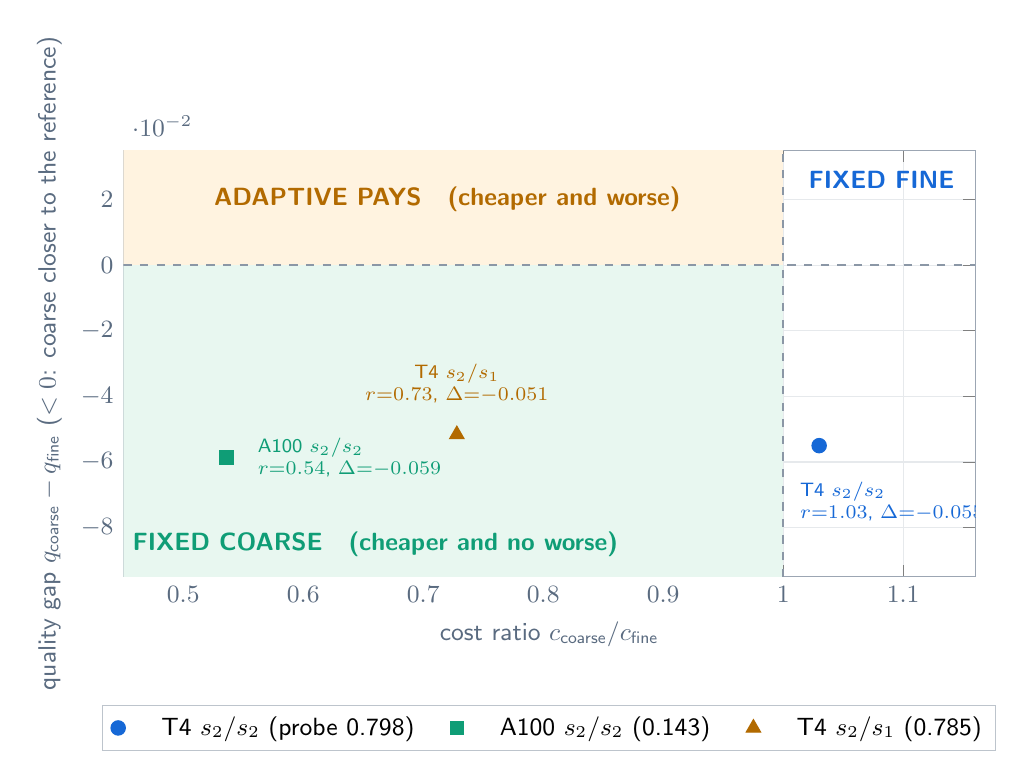
\begin{tikzpicture}
\begin{axis}[
  width=12.4cm, height=7.0cm,
  xlabel={cost ratio  $c_{\text{coarse}}/c_{\text{fine}}$},
  ylabel={quality gap  $q_{\text{coarse}}-q_{\text{fine}}$  ($<0$: coarse closer to the reference)},
  xmin=0.45, xmax=1.16, ymin=-0.095, ymax=0.035,
  axis line style={draw=mut!60},
  tick label style={font=\small,color=mut},
  label style={font=\small,color=mut},
  grid=major, grid style={draw=mut!15},
  legend style={font=\small,at={(0.5,-0.30)},anchor=north,legend columns=3,
                draw=mut!40,fill=white,column sep=1.1em},
]

% ---- shaded regions ----
\fill[payfill]  (axis cs:0.45,0)      rectangle (axis cs:1.0,0.035);
\fill[goodfill] (axis cs:0.45,-0.095) rectangle (axis cs:1.0,0);
\node[font=\small\bfseries,color=orangec,align=center] at (axis cs:0.72,0.020)
  {ADAPTIVE PAYS \; (cheaper \emph{and} worse)};
\node[font=\small\bfseries,color=greenc,align=center] at (axis cs:0.66,-0.085)
  {FIXED COARSE \; (cheaper and no worse)};
\node[font=\small\bfseries,color=bluec,align=center] at (axis cs:1.082,0.026)
  {FIXED FINE};

% ---- boundary lines ----
\draw[mut!70,dashed,line width=0.5pt] (axis cs:1.0,-0.095) -- (axis cs:1.0,0.035);
\draw[mut!70,dashed,line width=0.5pt] (axis cs:0.45,0) -- (axis cs:1.16,0);

% ---- operating points ----
\addplot[only marks,mark=*,mark size=2.6pt,color=bluec]
  coordinates {(1.030,-0.0550)};
\addplot[only marks,mark=square*,mark size=2.4pt,color=greenc]
  coordinates {(0.536,-0.0586)};
\addplot[only marks,mark=triangle*,mark size=3.0pt,color=orangec]
  coordinates {(0.728,-0.0516)};
\legend{T4 $s_2/s_2$ (probe 0.798), A100 $s_2/s_2$ (0.143), T4 $s_2/s_1$ (0.785)}

% ---- point labels, disambiguated: r = cost ratio, Delta = quality gap ----
% (an earlier draft labelled these "small gap" / "large gap", which referred to the
%  cost gap on the x-axis rather than the plotted quality gap on the y-axis.)
\node[font=\scriptsize,color=bluec,anchor=north west,align=left] at (axis cs:1.006,-0.063)
  {T4 $s_2/s_2$\\$r{=}1.03$, $\Delta{=}{-}0.055$};
\node[font=\scriptsize,color=greenc,anchor=west,align=left] at (axis cs:0.554,-0.0586)
  {A100 $s_2/s_2$\\$r{=}0.54$, $\Delta{=}{-}0.059$};
\node[font=\scriptsize,color=orangec,anchor=south,align=center] at (axis cs:0.728,-0.045)
  {T4 $s_2/s_1$\\$r{=}0.73$, $\Delta{=}{-}0.051$};

\end{axis}
\end{tikzpicture}
\end{document}
